%%%%%%%%%%%%%%%%%%%%%%%%%%%%%%%%%%%%%%%%%%%%%%%%%%%%%%%%%%%%%%%%%%%%%%
%% STEM-Alt: An Adversarial Generator-Critic Loop with Human-Aligned
%% Review for STEM Alt-Text.
%%
%% Course paper for 376-1230-00L Digital Accessibility, ETH Zurich,
%% FS2026. Uses the Springer Nature article template (v3.1, December
%% 2024), Math and Physical Sciences numbered reference style.
%%%%%%%%%%%%%%%%%%%%%%%%%%%%%%%%%%%%%%%%%%%%%%%%%%%%%%%%%%%%%%%%%%%%%%

\documentclass[pdflatex,sn-mathphys-num]{sn-jnl}

\usepackage{graphicx}
% Corpus-characterisation figures live in ../manuscript/figures and the
% clearly-labelled synthetic pipeline-preview figures in ../demo/figures, so
% both folders are on the graphics path and figures resolve by file name.
\graphicspath{{../manuscript/figures/}{../demo/figures/}}
\usepackage{multirow}
\usepackage{amsmath,amssymb,amsfonts}
\usepackage{amsthm}
\usepackage{mathrsfs}
\usepackage[title]{appendix}
\usepackage{xcolor}
\usepackage{textcomp}
\usepackage{manyfoot}
\usepackage{booktabs}
\usepackage{algorithm}
\usepackage{algorithmicx}
\usepackage{algpseudocode}
\usepackage{listings}
\usepackage[utf8]{inputenc}

% Supply an ASCII PDF metadata title that hyperref can encode without
% generating "Token not allowed in a PDF string" warnings.
\hypersetup{
  pdftitle={STEM-Alt: An Adversarial Generator-Critic Loop with Human-Aligned Review for STEM Alt-Text}
}

% Silence cosmetic SN-template artefacts that do not affect output:
%   - rsfs script-font size substitutions (the SN class loads mathrsfs for
%     theorem styling; LaTeX auto-substitutes the closest available size).
%   - hyperref bookmark-level differences caused by the SN class's
%     \bmhead{...} backmatter macros (Acknowledgements, Data availability,
%     Code availability). These do not affect the rendered PDF body.
\usepackage{silence}
\WarningFilter{latexfont}{Font shape `U/rsfs/m/n'}
\WarningFilter{latexfont}{Size substitutions with differences}
\WarningFilter{hyperref}{Difference}

\raggedbottom

\begin{document}

\title[STEM-Alt: Generator--Critic Loop for STEM Alt-Text]{STEM-Alt: An Adversarial Generator--Critic Loop with Human-Aligned Review for STEM Alt-Text}

\author*[1,2,3]{\fnm{Arvid E.} \sur{Gollwitzer}}\email{arvidg@mit.edu}

\affil*[1]{\orgdiv{Department of Electrical Engineering and Computer Science}, \orgname{Massachusetts Institute of Technology}, \orgaddress{\city{Cambridge}, \postcode{02139}, \state{MA}, \country{USA}}}

\affil[2]{\orgname{Broad Institute of MIT and Harvard}, \orgaddress{\city{Cambridge}, \postcode{02142}, \state{MA}, \country{USA}}}

\affil[3]{\orgname{ETH Z\"urich}, \orgaddress{\city{Z\"urich}, \country{Switzerland}}}

\abstract{Most scientific figures on the web carry no equivalent text alternative. Multimodal large language models cannot fill that gap, because the screen-reader user cannot verify a confidently wrong description. At the scale of a university course catalogue, human review is the bottleneck: rating every figure in every STEM course every semester is infeasible. We present \textbf{STEM-Alt}, a generator, critic, and human loop that converts a small set of dual human ratings into a domain-specific open-weights critic for STEM alt-text. The critic is LLaVA-Next-7B with rank-16 LoRA adapters, fine-tuned on 120 figures stratified across four STEM domains and the four ETH alt-text categories. The generator $G$ is drawn from three closed-API multimodal systems (GPT-4o, Claude 3.7 Sonnet, Gemini 2.5 Pro) under two prompting regimes (P1 generic, P2 WCAG-aware). The three systems and two regimes together yield 900 candidate alt-texts. The inner loop runs $k = 5$ rounds per figure. The convergence target is Krippendorff's $\alpha \geq 0.7$ between the calibrated critic $C$ and the human raters $H$ on a 30-figure held-out split. The target must hold across two consecutive Direct Preference Optimization rounds. The released artefact has four parts: an open-weights LoRA checkpoint, a CC-BY corpus, a born-accessible reference implementation validated against the DIAGRAM Image Description Guidelines and WCAG 2.2 SC 1.1.1, and the protocol an ETH course team can run on its existing figure backlog. The calibrated critic is positioned as an assistant, not as an arbiter, following Lecture 12 of the ETH Digital Accessibility course. Human review remains authoritative on the calibration split. The reproducibility guarantee belongs to the open-weights critic, not to the closed-API generators.}

\keywords{alt-text, scientific figures, WCAG 2.2, DIAGRAM, vision--language models, LLM-as-judge, Direct Preference Optimization, screen-reader users, accessibility}

\maketitle

%%%%%%%%%%%%%%%%%%%%%%%%%%%%%%%%%%%%%%%%%%%%%%%%%%%%%%%%%%%%%%%%%%%%%%
\section{Introduction}\label{sec:intro}

A blind or low-vision student encountering a STEM figure has one chance to learn from it: the text alternative. If the alt-text is wrong, the student cannot tell. WCAG 2.2 Success Criterion 1.1.1 \cite{wcag22nontext} makes the alt-text mandatory. STEM teaching routinely fails it because the figures carry the information and writing equivalent text is hard. Multimodal large language models can draft alt-text quickly, yet on scientific content their drafts fail in ways the affected reader cannot verify. Lecture 12 of the ETH Digital Accessibility course \cite{bolfingHeim2026Lecture12} names three structural reasons. Training data on complex, novel scientific content is sparse, so AI interpretations are sometimes highly flawed. Trust collapses when the reader cannot audit the output. And outsourcing accessibility to AI pushes the inclusion burden back onto the affected individual, against the lecture's principle that ``accessibility is the prerequisite for good AI, not its result''.

Human review is the bottleneck. Human-rated alt-text is the gold standard, but no human team rates every figure in every ETH course every semester. Static benchmarks measure the gap; they do not close it.

We introduce \textbf{STEM-Alt}, a generator, critic, and human loop that amortises human judgement across the long tail of figures (Fig.~\ref{fig:overview}). A small dual-rated calibration set teaches an open-weights critic to score alt-text the way the human raters do. The calibrated critic then scores AI-generated alt-text on the remaining figures with only sparse human oversight. The critic is an assistant, not an arbiter, in the lecture's sense of ``always my assistant, never in charge'' \cite{bolfingHeim2026Lecture12}. Human ratings remain authoritative on the calibration split. The critic extends that judgement to the long tail only under a falsifiable convergence criterion.

\begin{figure}[!t]
\centering
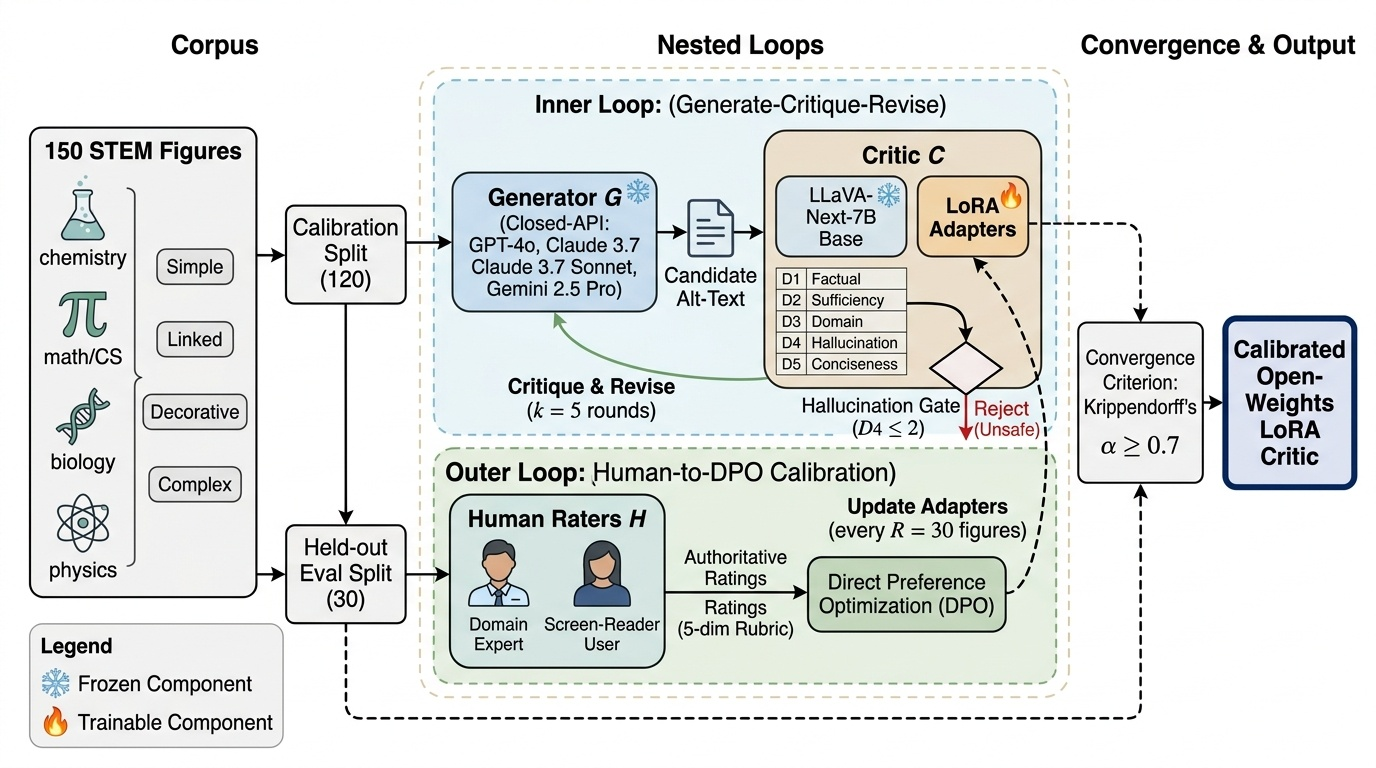
\includegraphics[width=\textwidth]{fig_overview.png}
\caption{Overview of the STEM-Alt human-aligned self-correction loop for scientific-figure alt-text. Schematic pipeline diagram, read left to right. A corpus of 150 openly licensed STEM figures, stratified by domain and ETH category, is partitioned into a 120-figure calibration split and a 30-figure held-out split. In the inner loop, a closed-API generator $G$ (GPT-4o, Claude 3.7 Sonnet, or Gemini 2.5 Pro) drafts a candidate alt-text. The open-weights critic $C$ (LLaVA-Next-7B with rank-16 LoRA adapters) scores it on the five-dimension rubric and returns a one-paragraph critique, and $G$ revises, for $k = 5$ rounds or until the score plateaus. On the calibration split, a human $H$ rates the final alt-text on the same rubric. Here $H$ is a domain expert and a screen-reader user listening through NVDA. In the outer loop, every $R = 30$ figures the accumulated critic--human score pairs fine-tune $C$ with Direct Preference Optimization. Training stops when the critic--human Krippendorff $\alpha$ meets the pre-registered convergence criterion on the held-out split ($\alpha \geq 0.7$, sustained over two consecutive DPO rounds). The released artefact is the calibrated open-weights critic: the base model is frozen and only the LoRA adapters are trainable.}\label{fig:overview}
\end{figure}

\textbf{Contributions.} (1)~A domain-specific calibrated critic for STEM alt-text, released as an open-weights LoRA checkpoint on LLaVA-Next-7B. (2)~A falsifiable convergence criterion: Krippendorff's $\alpha$ between critic and human on a held-out 30-figure split, monotonic improvement across DPO rounds, and a $0.7$ threshold sustained across two consecutive rounds. (3)~A born-accessible reference implementation aligned with the DIAGRAM Image Description Guidelines \cite{diagramGuidelines2019}, the DIAGRAM Accessible Image Sample Book \cite{diagramSampleBook2019}, and the ETH four-category alt-text taxonomy \cite{ethStaffnetAltText,ethStaffnetComplexExamples}. (4)~A characterisation of the minimum human budget required to reach the tolerance, and a residual-disagreement profile by domain, category, and rubric dimension.

STEM-Alt does not propose a new optimisation algorithm. It packages an existing one (DPO) and an existing critic family (LLaVA-Next-7B with LoRA) into a domain-specific calibrated artefact that an ETH course team can run on its existing figure backlog. The contribution is the artefact, not the algorithm.

%%%%%%%%%%%%%%%%%%%%%%%%%%%%%%%%%%%%%%%%%%%%%%%%%%%%%%%%%%%%%%%%%%%%%%
\section{Background and Related Work}\label{sec:related}

Two literatures bear directly on STEM-Alt: LLM-as-judge calibration and accessibility-compliant alt-text generation. LLM-as-judge has become a standard evaluation approach in language modelling, with MT-Bench \cite{zheng2023mtbench}, G-Eval \cite{liu2023geval}, JudgeLM \cite{zhu2023judgelm}, and Prometheus \cite{kim2024prometheus} the canonical examples. These methods calibrate general-purpose judges on general text distributions. STEM-Alt instead narrows the target to a specific domain (STEM figures), a specific evaluator (open-weights LLaVA-Next-7B \cite{llavaNext2024}), and a specific update path (DPO \cite{rafailov2023dpo} from in-domain dual human ratings). The judge does not need to be universal. It needs to be reliable in distribution.

The optimisation route is chosen for sample efficiency, not for novelty. We use DPO \cite{rafailov2023dpo} rather than full RLHF \cite{christiano2017deeprlhp} on a small calibration set, and LoRA \cite{hu2022lora} so that fine-tuning a 7B vision--language model stays tractable on a single GPU. Closed-API generators drift across versions, so the reproducibility guarantee belongs to the open-weights critic only. Section~\ref{subsec:dpo} gives the technical detail.

Compliance follows four normative sources. The DIAGRAM Image Description Guidelines \cite{diagramGuidelines2019} and the DIAGRAM Accessible Image Sample Book \cite{diagramSampleBook2019} fix the format and figure-type taxonomy. The ETH ``Text Alternatives'' guidance \cite{ethStaffnetAltText} fixes the four-category split (simple, linked, decorative, complex). WCAG 2.2 SC 1.1.1 \cite{wcag22nontext} is the normative gate. Every gold-standard description and every loop output meets these standards. An automated linter enforces compliance at corpus build time, and human raters reject any output that fails the same rules at rating time.

%%%%%%%%%%%%%%%%%%%%%%%%%%%%%%%%%%%%%%%%%%%%%%%%%%%%%%%%%%%%%%%%%%%%%%
\section{Method}\label{sec:method}

\subsection{Corpus}\label{subsec:corpus}

The corpus is designed to expose the critic to every cell of the ETH-category by STEM-domain matrix. It also keeps a held-out slice that the loop never sees. It contains 150 openly licensed figures drawn from OpenStax, MIT OpenCourseWare, arXiv CC-BY, and Wikimedia Commons. We partition the corpus at the start into a \textbf{calibration split} of 120 figures (loop and DPO fine-tuning) and a \textbf{held-out evaluation split} of 30 figures (never used for fine-tuning). Stratification runs along two axes: STEM domain (chemistry, mathematics and computer science, biology, physics) and ETH alt-text category (simple, linked, decorative, complex). Each entry carries the source URL, the licence, the domain, the ETH category, the DIAGRAM image type, an expert reference description, a short alt, and the surrounding context paragraph from the source. The released subset (Table~\ref{tab:corpus}, Fig.~\ref{fig:strat}) is the held-out 30 figures plus their metadata. It serves as the primary external evaluation set for downstream users of the critic.

\begin{figure}[!htb]
\centering
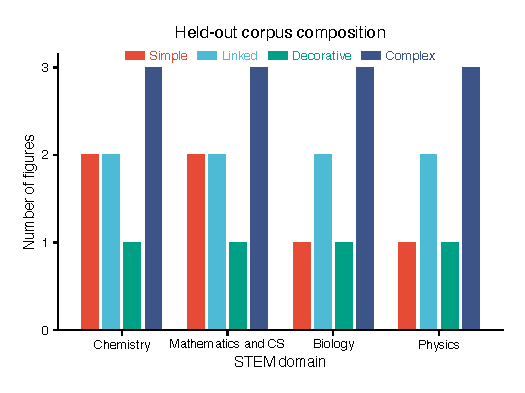
\includegraphics[width=0.82\textwidth]{fig_corpus_stratification_pub.pdf}
\caption{Composition of the released 30-figure held-out corpus. Grouped bar chart of the number of figures by STEM domain (chemistry, mathematics and computer science, biology, physics), with one bar per ETH alt-text category (simple, linked, decorative, complex). Chemistry and mathematics and computer science hold eight figures each (two simple, two linked, one decorative, three complex); biology and physics hold seven each (one simple, two linked, one decorative, three complex). Complex figures dominate (12 of 30) by design, because they are where AI alt-text fails hardest and where the critic is most needed.}\label{fig:strat}
\end{figure}

\begin{table}[!htb]
\caption{Held-out evaluation split, stratified by STEM domain and ETH alt-text category. Cells give the count of figures.}\label{tab:corpus}
\centering
\begin{tabular}{lrrrrr}
\toprule
Domain & Simple & Linked & Decorative & Complex & Total \\
\midrule
Chemistry & 2 & 2 & 1 & 3 & 8 \\
Mathematics and computer science & 2 & 2 & 1 & 3 & 8 \\
Biology & 1 & 2 & 1 & 3 & 7 \\
Physics & 1 & 2 & 1 & 3 & 7 \\
\midrule
\textbf{Total} & \textbf{6} & \textbf{8} & \textbf{4} & \textbf{12} & \textbf{30} \\
\bottomrule
\end{tabular}
\end{table}

\textbf{Corpus characterisation.} Three descriptive properties of the released split are reported directly from the manifest by \texttt{analysis/analyze\_corpus.py}, and each ships with the CSV it was rendered from. First, the corpus spans nine DIAGRAM figure types. Graphs (8) and relational diagrams (7) are the most frequent, matching the structure-heavy content of STEM teaching material. Second, all 30 figures are openly licensed. The 28 reused third-party images are public domain (17), CC-BY-SA-3.0 (8), CC-BY-SA-4.0 (2), and CC-BY-3.0 (1). The two mathematics-and-computer-science complex figures, a loss landscape and a longest-common-subsequence table, are rendered locally and released by the author under CC-BY 4.0. Third, the corpus satisfies its own compliance claim. The four decorative figures carry an empty short alt by design. The 26 non-decorative figures have short alts of 17 to 53 characters (median 31.5). None exceeds the DIAGRAM \S A.3 125-character bound, so the violation set is empty. Appendix~\ref{app:corpus} gives the per-type, per-licence, and short-alt-length distributions as figures.

\subsection{\texorpdfstring{Generator $G$}{Generator G}}\label{subsec:generator}

The generator $G$ is drawn from three closed-API frontier multimodal systems: GPT-4o, Claude 3.7 Sonnet, and Gemini 2.5 Pro. Closed-API outputs drift across versions, so the reproducibility guarantee is carried by the open-weights critic rather than by the generators. The critic's LLaVA-Next-7B backbone can be pinned at a model revision for exact re-runs.

Two prompts are used. \textbf{P1 (generic)} is the one-line instruction ``Provide alt-text for this image suitable for a blind reader.'' \textbf{P2 (WCAG-aware)} names the four ETH categories and asks $G$ to classify the figure before describing it. The output then conforms to the ETH-category contract: a concise alt for simple or linked figures, an empty alt attribute for decorative figures, and a short alt plus a long description for complex figures. P2 embeds the DIAGRAM general rules and shows one Sample Book chapter as a one-shot example. Inside the loop, $G$ receives $C$'s score and short critique and revises. Temperature is fixed at 0. Prompts, model versions, decoding parameters, and timestamps are logged for every candidate. Across the full 150-figure corpus, the three generators under two prompting regimes produce $3 \times 2 \times 150 = 900$ candidate alt-texts.

\subsection{\texorpdfstring{Critic $C$}{Critic C}}\label{subsec:critic}

The critic $C$ is LLaVA-Next-7B with rank-16 LoRA adapters on the attention query, key, value, and output projections. We freeze the base model and train only the adapters between rounds. $C$ receives the image, the candidate alt-text, the surrounding context paragraph, and the DIAGRAM figure type. It then emits five-dimension scores plus a one-paragraph critique:

\begin{table}[!htb]
\caption{Five-dimension rubric. $D_1$--$D_3$ form the primary outcome.}\label{tab:rubric}
\centering
\small
\begin{tabular}{cll}
\toprule
Dim. & Name & Definition \\
\midrule
$D_1$ & Factual correctness & Does the description correctly state what is visible? \\
$D_2$ & Information sufficiency & Enough to reconstruct the figure's claim? \\
$D_3$ & Domain accuracy & Are technical terms used correctly in the figure's field? \\
$D_4$ & Hallucination & Does the description add content not in the figure? \\
$D_5$ & Conciseness & Does it follow DIAGRAM length guidance for its category? \\
\bottomrule
\end{tabular}
\end{table}

Each dimension is scored on a 5-point Likert scale (1 = poor, 5 = excellent). The primary outcome is the mean of $D_1, D_2, D_3$, the dimensions most directly tied to factual screen-reader utility.

\subsection{The loop}\label{subsec:loop}

For each figure, the loop runs: (1)~$G$ produces alt-text under P2; (2)~$C$ scores and returns a short critique; (3)~$G$ revises against the critique; (4)~steps 2--3 repeat for $k = 5$ inner rounds, or until $C$'s score plateaus ($\Delta$ on the primary outcome below $0.1$ between consecutive rounds); (5)~$H$ rates the final alt-text on calibration-split figures.

\subsection{DPO fine-tuning}\label{subsec:dpo}

DPO is chosen over full RLHF for sample efficiency. The calibration set yields only $\sim 2{,}400$ preference pairs, well below the regime where a learned reward model is reliable. DPO's closed-form objective on preference pairs eliminates one source of approximation error and one stage of training. Every $R = 30$ newly calibrated figures, we fine-tune $C$ on the accumulated $(C\text{-score}, H\text{-score})$ pairs. We construct preference pairs by ranking within-figure candidates by $H$-score. Each figure yields 4 candidates, hence $\binom{4}{2} = 6$ pairs, giving $6 \times 30 = 180$ in-figure pairs per fine-tuning round. Across the four fine-tuning rounds of the 120-figure calibration set this gives 720 within-figure pairs. Between-round comparisons augment that to roughly $2{,}400$. The DPO objective \cite{rafailov2023dpo} is
\begin{equation}
\mathcal{L}_{\mathrm{DPO}}(C) = -\,\mathbb{E}_{(x,y^+,y^-)\sim \mathcal{D}_{\mathrm{pref}}}\!\left[ \log \sigma\!\left( \beta \bigl( r_C(x,y^+) - r_C(x,y^-) \bigr) \right) \right],
\label{eq:dpo}
\end{equation}
where $x$ is the context tuple (image, surrounding paragraph, DIAGRAM figure type), $y^+$ is the human-preferred candidate, $y^-$ is dispreferred, $r_C(x,y) = \log \frac{\pi_C(y\mid x)}{\pi_{\mathrm{ref}}(y\mid x)}$ is $C$'s implicit reward against the frozen reference policy, $\sigma$ is the sigmoid, and $\mathcal{D}_{\mathrm{pref}}$ is the preference dataset. We use $\beta = 0.1$.

We make three assumptions explicit. \emph{Reward identifiability}: zero-initialised LoRA adapters give $\pi_C \equiv \pi_{\mathrm{ref}}$ at $r=0$, so $r_C \equiv 0$ there. The DPO gradient then depends only on $y^+, y^-$. \emph{Pair independence}: in-figure pairs are conditionally independent given $x$. Between-round pairs (the same figure across rounds) are positively correlated, so we down-weight them by $\lambda = 0.3$ in the loss. \emph{Scale}: $\alpha$ is computed under interval-scale assumptions \cite{hayes2007krippendorff}, with ordinal-scale $\alpha$ reported as a robustness check.

\textbf{Stopping criterion.} $\alpha \geq 0.7$ between $C$ and $H$ on the primary outcome (mean of $D_1, D_2, D_3$), sustained across two consecutive fine-tuning rounds on the held-out split.

\subsection{Human protocol}\label{subsec:human}

Two raters score each calibration figure. The first is a \textbf{domain expert} with research-level fluency in the figure's STEM area. The second is a \textbf{screen-reader user} (recruited through Stiftung Zugang f\"ur alle) who listens to the alt-text rendered with NVDA at standard rate before rating. Both raters use the same five-dimension rubric on the same 5-point scale, and raters do not see $C$'s scores. The rubric is piloted on a 20-figure subset, disagreements are adjudicated, and the rubric is frozen before scaling. An inter-rater reliability floor of Krippendorff's $\alpha \geq 0.6$ between $H_1$ and $H_2$ on the primary outcome is required. Figures whose ratings fall below the floor are adjudicated rather than entering the calibration set. The $C$--$H$ convergence threshold (\S\ref{subsec:dpo}, $\alpha \geq 0.7$) is the separate downstream criterion the loop must meet on the held-out split. The minimum-human-budget claim is the smallest number of human-rated figures at which the convergence tolerance is reached on the held-out split.

\subsection{Baselines}\label{subsec:baselines}

We benchmark against four baselines that isolate each contribution. \textbf{B1} is single-shot $G$ under P1, with no loop and no critic. \textbf{B2} is a prompt-only loop in which $G$ under P2 self-revises against its own previous draft, again with no critic. \textbf{B3} is the frozen critic: $G$ paired with the base LLaVA-Next-7B under P2, with no DPO update. \textbf{B4} extends B3 with in-context examples of high- and low-rated alt-text in the critic prompt. \textbf{STEM-Alt (ours)} is the full loop with the DPO-fine-tuned critic.

%%%%%%%%%%%%%%%%%%%%%%%%%%%%%%%%%%%%%%%%%%%%%%%%%%%%%%%%%%%%%%%%%%%%%%
\section{Evaluation}\label{sec:eval}

The evaluation plan below is pre-registered. The thresholds, statistics, and figures are fixed in advance. At this stage the released artefact is the characterised held-out corpus (\S\ref{subsec:corpus}, Appendix~\ref{app:corpus}). The convergence numbers will follow once the human-rating study (Appendix~\ref{app:human}) and the GPU fine-tuning run complete. The evaluation harness is implemented and unit-tested. It emits four figures from the held-out report: a \emph{convergence curve} (critic--human $\alpha$ against DPO round, against the $0.7$ sustained-for-two-rounds threshold), a \emph{critic--human scatter} (per-figure $C$ versus $H$ primary-outcome score against the perfect-agreement diagonal), a \emph{per-dimension agreement} bar chart ($C$--$H$ $\alpha$ for each of $D_1$--$D_5$ at the final round), and a \emph{residual-disagreement heatmap} (mean absolute $C$--$H$ difference by domain and category). To exercise the renderer and the report schema before the study runs, the harness is also driven by a seeded synthetic preview. The convergence curve and the critic--human scatter on that preview are shown below (Figs~\ref{fig:demo-conv} and~\ref{fig:demo-scatter}), and the per-dimension agreement and residual-disagreement figures are in Appendix~\ref{app:harness}. The preview illustrates format and plumbing only and carries no findings. We will report the convergence $\alpha$ as a measured result only after the real study replaces the preview.

\textbf{Primary outcome.} Krippendorff's $\alpha$ \cite{hayes2007krippendorff,krippendorff2011alpha} between $C$ and $H$ on the mean of $D_1, D_2, D_3$, computed at each fine-tuning round $r$ on the held-out split. The convergence threshold is $\alpha \geq 0.7$ sustained for two consecutive $r$.

\textbf{Convergence curve.} Critic--human $\alpha$ on the primary outcome against $r$, shown with the $0.7$ sustained-for-two-rounds threshold and figure-stratified bootstrap 95\% confidence intervals ($B = 2{,}000$ resamples). The mean absolute $C$--$H$ score difference against $r$ is tracked as a companion diagnostic.

\begin{figure}[!htb]
\centering
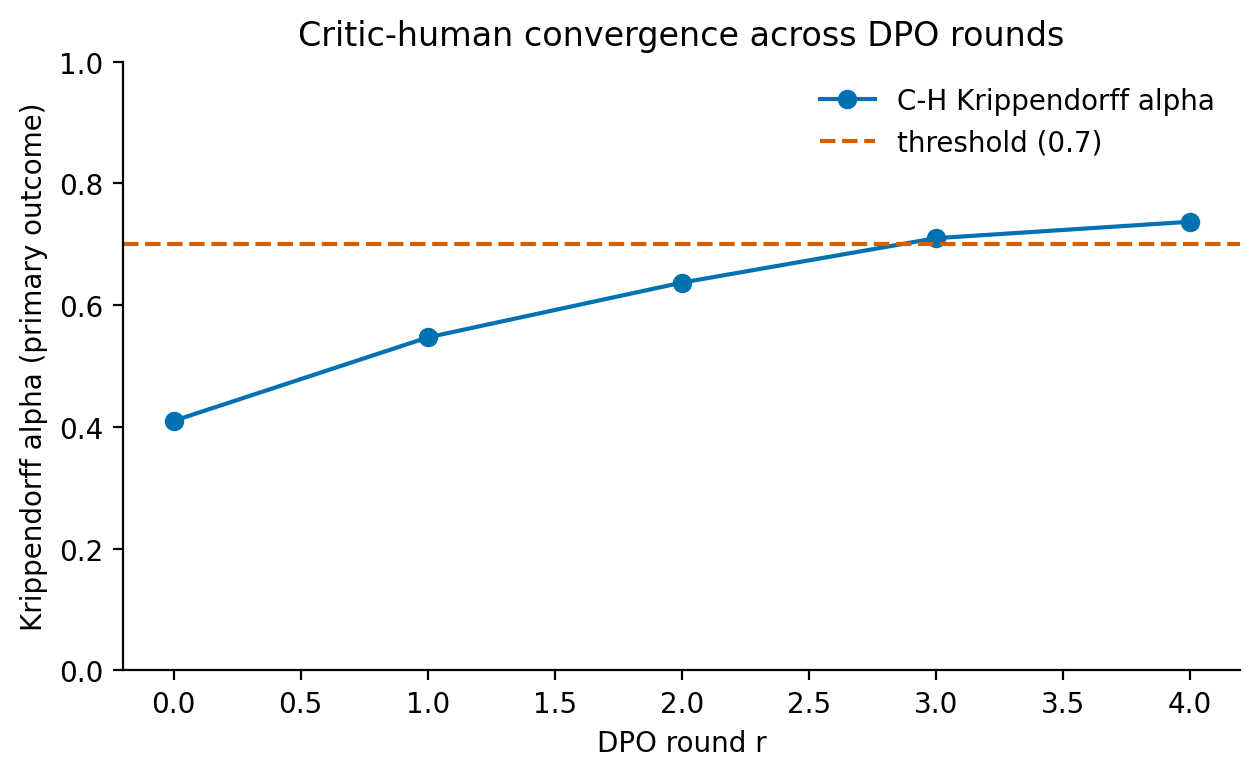
\includegraphics[width=0.8\textwidth]{fig_convergence_curve.png}
\caption{Synthetic pipeline preview, not a measured result. Convergence-curve layout: the critic--human Krippendorff $\alpha$ on the primary outcome ($y$ axis) against the DPO round ($x$ axis), with a dashed reference line at the $0.7$ threshold. The shape is the pre-registered analysis; the plotted values are simulated placeholders from a seeded preview (\S\ref{app:harness}), not measured agreement.}\label{fig:demo-conv}
\end{figure}

\begin{figure}[!htb]
\centering
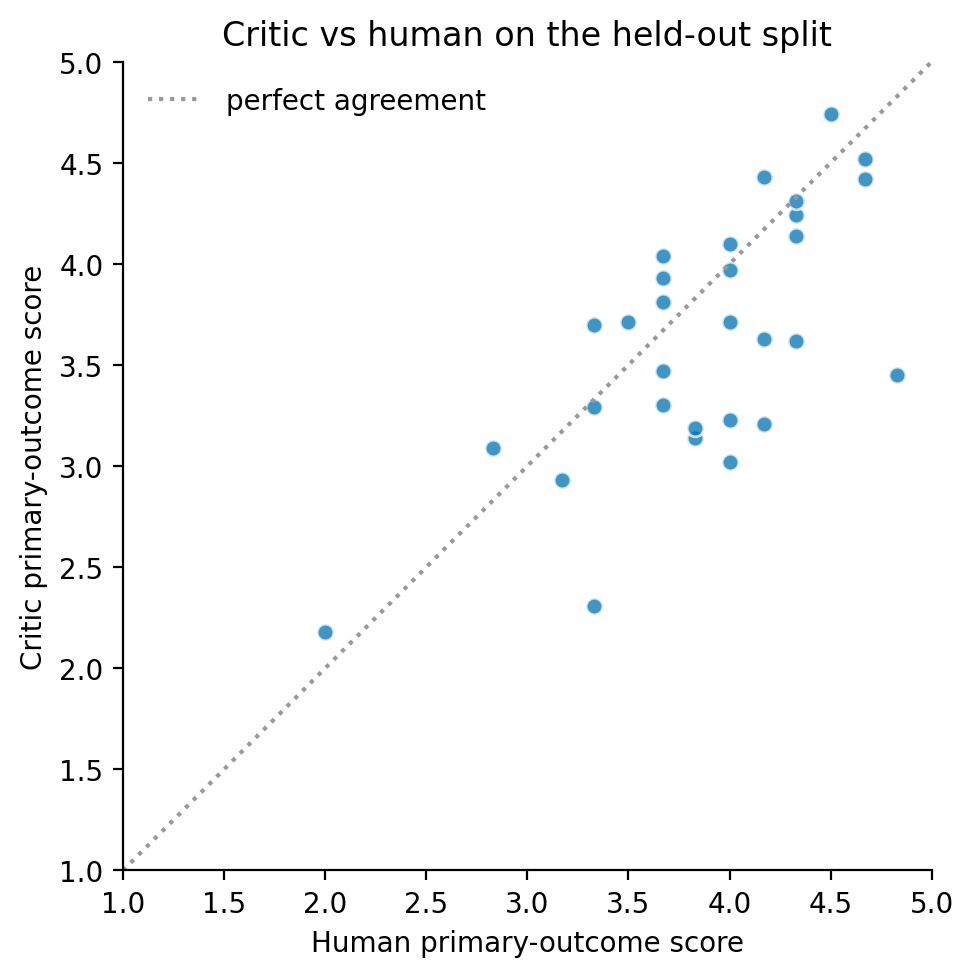
\includegraphics[width=0.8\textwidth]{fig_ch_scatter.png}
\caption{Synthetic pipeline preview, not a measured result. Critic--human scatter layout: the critic score against the human score for each held-out figure, with a diagonal line of perfect agreement. The shape is the pre-registered analysis; the plotted values are simulated placeholders from a seeded preview (\S\ref{app:harness}), not measured agreement.}\label{fig:demo-scatter}
\end{figure}

\textbf{Iteration effect.} Paired comparison of $H$'s rating on $G$'s single-shot output (P1, no loop) versus the $k$-round loop output (P2 with critic). A mixed-effects linear model treats figure as a random intercept and treatment as a fixed effect.

\textbf{Generalisation.} $C$'s $\alpha$ is reported on three held-out conditions: \emph{G1} unseen subjects within trained categories; \emph{G2} unseen DIAGRAM categories; \emph{G3} unseen STEM domains.

\textbf{Human budget.} The sample-efficiency curve plots held-out $\alpha$ as a function of human-rated figures used in DPO. A non-parametric LOWESS fit identifies the minimum-budget inflection point.

\textbf{Power.} With 30 held-out figures $\times$ 2 raters $\times$ 5 dimensions $= 300$ ratings, a paired two-sided test at $\gamma = 0.05$ has power $0.80$ to detect a Krippendorff $\alpha$ shift of $0.15$. Power is computed with the bootstrap variance estimator from Hayes and Krippendorff \cite{hayes2007krippendorff}.

\textbf{Notation.} $G,C,H$ = generator, critic, human; $r$ = DPO round, $k$ = inner round per figure; $\alpha$ = Krippendorff's alpha; $\beta$ = DPO regularisation; $\gamma$ = significance level; $\pi_C, \pi_{\mathrm{ref}}$ = critic and frozen reference policy; $\lambda$ = between-round pair weight.

%%%%%%%%%%%%%%%%%%%%%%%%%%%%%%%%%%%%%%%%%%%%%%%%%%%%%%%%%%%%%%%%%%%%%%
\section{Compliance and Born-Accessible Release}\label{sec:compliance}

Compliance is gated, not aspired. An automated linter rejects any gold-standard description that fails the DIAGRAM style rules. Human raters reject any loop output that fails the same rules. Compliance failure counts as a generation error, not as a rating dimension.

The DIAGRAM general rules \cite{diagramGuidelines2019} are enforced as follows. \S A.1 \emph{Context is key}: every figure ships with its surrounding context paragraph, and descriptions assume the context rather than duplicating the caption. \S A.2 \emph{Audience-aware}: the audience is fixed at ``blind or low-vision STEM reader, undergraduate to research level''. \S A.3 \emph{Concise}: short alt is bounded at 125 characters where the image type permits, and captioned figures point to the caption. \S A.4 \emph{Objective}: descriptions report what is visible, with no pedagogical interpretation. \S A.5 \emph{General to specific}: every long description opens with a one-sentence summary and then drills down. \S A.6 \emph{Tone}: active verbs, present tense, and abbreviations spelled out where pronunciation matters. \S B \emph{Inset handling}: embedded graphs render as row-and-column data tables when a one-sentence summary is insufficient.

The paper is released as a born-accessible PDF: PDF/UA is the accessibility target, and the build is checked with the PAC PDF/UA checker before publication. The same sources can optionally render to two other channels for readers who prefer them. One is semantic HTML (ARIA landmarks, a validated heading hierarchy, and an \texttt{axe-core} audit). The other is an EPUB3 build following the Sample Book structure.

\subsection{Failure modes and concrete mitigations}\label{subsec:mitigations}

Four failure modes can introduce information that misleads a screen-reader user. Each is paired with a concrete mitigation enforced inside the loop or at rating time.

\emph{Hallucination.} The description states content not visible in the figure. This is the most damaging failure mode for a reader who cannot verify the description. \textbf{Mitigation:} dimension $D_4$ scores hallucination explicitly on the five-point rubric, and $D_4 \leq 2$ triggers automatic rejection of the candidate inside the loop. Any candidate that survives to release also passes the human rater's $D_4$ check.

\emph{Category misclassification.} The generator treats a complex figure as a simple one, producing under-described content. \textbf{Mitigation:} P2 requires $G$ to classify the figure before describing it, and the compliance linter rejects outputs whose format does not match the declared category.

\emph{Length violation.} The alt-text is excessive or insufficient, burdening screen-reader navigation. \textbf{Mitigation:} dimension $D_5$ enforces DIAGRAM §A.3 length guidance, and the linter applies the 125-character short-alt bound where the image type permits.

\emph{Pedagogical or interpretive injection.} The description states what the figure ``means'' rather than what is visible, shifting authority away from the reader. \textbf{Mitigation:} DIAGRAM §A.4 (\emph{objective}) is enforced by the linter and by the human raters, and the rubric definition of $D_1$ ties factual correctness to what is visible, not to what is implied.

Cases that survive all four mitigations and still mislead are reported as residual-disagreement events in the held-out evaluation, broken down by domain, category, and dimension.

%%%%%%%%%%%%%%%%%%%%%%%%%%%%%%%%%%%%%%%%%%%%%%%%%%%%%%%%%%%%%%%%%%%%%%
\section{Limitations}\label{sec:limitations}

Three limitations bound the strength of the claims.

\textbf{(1) Calibration set size and inter-rater ceiling.} The 120-figure calibration split yields roughly $2{,}400$ preference pairs (720 within-figure pairs, augmented by between-round comparisons), small relative to the 10K+ pairs used in production DPO. The achievable $C$--$H$ $\alpha$ cannot exceed the $H_1$--$H_2$ ceiling, since the critic is trained against the same two raters. We mitigate the small pair count by augmenting with between-round preference pairs. We report the sample-efficiency curve and the $H_1$--$H_2$ agreement explicitly, so the reader can locate the bottleneck.

\textbf{(2) Distribution-bound critic and frontier-model drift.} The critic is calibrated on STEM figures from open educational sources. Off-distribution use such as medical imaging, art history, or video frames requires re-calibration. Closed-API generator outputs drift across versions, so the reproducibility guarantee belongs to the open-weights critic and not to the generators that produced its training distribution.

\textbf{(3) Screen-reader-user availability.} Recruitment through Stiftung Zugang f\"ur alle is the primary path, recruitment via the WAI community is the backup, and a sighted rater with documented screen-reader experience is the disclosed fallback. We record which path each figure went through, so readers can stratify the reported $\alpha$ by rater provenance.

%%%%%%%%%%%%%%%%%%%%%%%%%%%%%%%%%%%%%%%%%%%%%%%%%%%%%%%%%%%%%%%%%%%%%%
\section{Conclusion}\label{sec:conclusion}

STEM-Alt is a generator, critic, and human loop that converts a small dual-rated calibration set into a domain-specific open-weights critic for STEM alt-text. The convergence criterion is falsifiable: Krippendorff's $\alpha \geq 0.7$ between $C$ and $H$ on the primary outcome, sustained over two consecutive DPO rounds on the held-out split. When the criterion holds, an ETH course team can extend scientific-figure accessibility across the remaining figures with only sparse human oversight, on its own open-weights infrastructure. The reproducibility guarantee belongs to the open-weights critic, not to the closed-API generators that populated its training distribution. Re-calibration is required outside STEM educational figures. The released artefact is a calibrated LoRA checkpoint, a CC-BY corpus, a born-accessible reference implementation, and the protocol for keeping the critic calibrated as content drifts.

\bmhead{Acknowledgements}

I sincerely thank Anton Bolfing and Manu Heim for the exceptional course. I am excited to continue this work.

\bmhead{Data availability}

The 30-figure held-out evaluation corpus is released as a structured manifest (\texttt{manifest.csv}). The 11 columns are \texttt{figure\_id}, \texttt{source\_url}, \texttt{licence}, STEM domain, ETH alt-text category, DIAGRAM figure type, expert reference description, short alt, context paragraph, \texttt{image\_path}, and \texttt{split}. The author releases four artefacts under CC-BY 4.0: the manifest, the held-out split (\texttt{splits.json}), the five-dimension rubric (\texttt{rubric.yaml}), and the two locally rendered figures (\texttt{mathcs\_complex\_loss\_landscape.png} and \texttt{mathcs\_complex\_dynamic\_programming.png}, rendered deterministically by \texttt{code/scripts/render\_local\_figures.py}). The 28 third-party figures are drawn from Wikimedia Commons, OpenStax (CC-BY 4.0), MIT OpenCourseWare, and arXiv (CC-BY 4.0). The manifest carries the source URL and the per-figure licence (public domain, CC-BY-SA-3.0, CC-BY-SA-4.0, CC-BY-4.0, or CC-BY-3.0). The licence-preserving figure files are acquired by running \texttt{pipeline/01\_build\_corpus.py} against the manifest. The 6-page manuscript and the 1- to 2-page accessible plain-language summary are released under CC-BY 4.0 as born-accessible PDFs (PDF/UA target). Semantic HTML and EPUB3 renderings can optionally be produced from the same sources.

The DPO-fine-tuned LLaVA-Next-7B LoRA checkpoint is the calibrated-critic artefact produced by the pipeline and is released in the same repository.\footnote{The rank-16 LoRA adapter is a small binary. It is versioned with Git LFS or attached as a release asset rather than committed inline.} Closed-API generator outputs are included subject to the academic-use terms of OpenAI, Anthropic, and Google; open-weights critic outputs are released under CC-BY 4.0.

All artefacts, including the fine-tuned checkpoint, are deposited in the project repository at \url{https://github.com/arvidgollwitzer/STEM-Alt}. There is no embargo, controlled-access committee, or commercial restriction on any released artefact. Please cite this manuscript when reusing any released artefact.

\bmhead{Code availability}

All code (the \texttt{stem\_alt} Python package, the Hydra configuration, the six-stage pipeline, the unit tests, and the build scripts) is released under the MIT licence at \url{https://github.com/arvidgollwitzer/STEM-Alt}. The release pins the dependency set in \texttt{code/pyproject.toml} and the random seed under \texttt{utils.set\_seed}. The run-config files pin the model versions used in the loop: the LLaVA-NeXT-7B revision and the GPT-4o, Claude 3.7 Sonnet, and Gemini 2.5 Pro snapshot strings.

\section*{Declarations}

\begin{itemize}
\item \textbf{Funding.} Not applicable.
\item \textbf{Conflict of interest.} The author declares no conflict of interest.
\item \textbf{Ethics approval and consent to participate.} Under this protocol, human ratings carry no personally identifying information beyond an opaque \texttt{rater\_id}, and recruitment goes through institutional channels.
\item \textbf{Data availability.} See the \emph{Data availability} section above.
\item \textbf{Code availability.} See the \emph{Code availability} section above.
\item \textbf{Author contribution.} Sole author; conceived, designed, implemented, and wrote the work.
\end{itemize}

\begin{appendices}

%%%%%%%%%%%%%%%%%%%%%%%%%%%%%%%%%%%%%%%%%%%%%%%%%%%%%%%%%%%%%%%%%%%%%%
\section{Corpus characterisation in detail}\label{app:corpus}
\setcounter{figure}{0}\setcounter{table}{0}

This appendix expands the corpus-characterisation summary of \S\ref{subsec:corpus}. Every value is emitted from \texttt{data/corpus/manifest.csv} by \texttt{analysis/analyze\_corpus.py}, and each figure ships with the CSV it was rendered from. The reproduced stratification matches the held-out split of Table~\ref{tab:corpus} exactly (\texttt{corpus\_summary.json}: \texttt{matches\_manuscript\_table1 = true}).

Table~\ref{tab:composition} gives the DIAGRAM figure-type and source-licence distributions, and Figs.~\ref{fig:diagtypes}--\ref{fig:shortalt} plot the three descriptive axes.

\begin{table}[!htb]
\caption{Composition of the 30 held-out figures by DIAGRAM figure type and by source licence.}\label{tab:composition}
\centering
\begin{tabular}{llr}
\toprule
Axis & Category & Count \\
\midrule
DIAGRAM figure type & Graphs & 8 \\
 & Relational diagrams & 7 \\
 & Illustrated diagrams & 4 \\
 & Photos & 4 \\
 & Chemistry & 2 \\
 & Tables & 2 \\
 & Mathematics & 1 \\
 & Art/photos/cartoons & 1 \\
 & Maps & 1 \\
\midrule
Source licence & Public domain & 17 \\
 & CC-BY-SA-3.0 & 8 \\
 & CC-BY-SA-4.0 & 2 \\
 & CC-BY-4.0 (local render) & 2 \\
 & CC-BY-3.0 & 1 \\
\bottomrule
\end{tabular}
\end{table}

\begin{figure}[!htb]
\centering
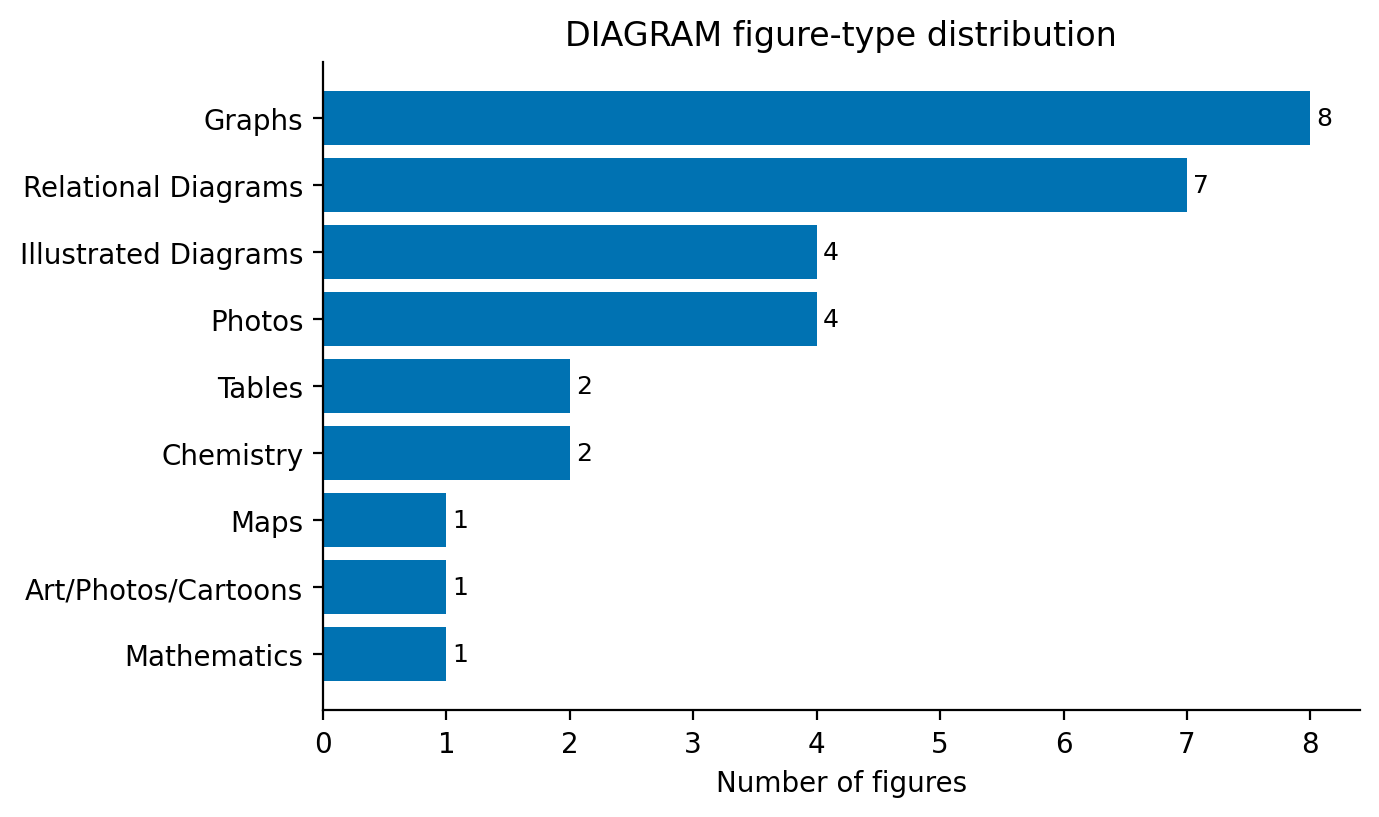
\includegraphics[width=0.86\textwidth]{fig2_diagram_types.png}
\caption{DIAGRAM figure-type distribution across the 30 held-out figures. Horizontal bar chart: graphs 8, relational diagrams 7, illustrated diagrams 4, photos 4, chemistry 2, tables 2, mathematics 1, art/photos/cartoons 1, maps 1. Graphs and relational diagrams dominate, matching the structure-heavy content of STEM teaching material.}\label{fig:diagtypes}
\end{figure}

\begin{figure}[!htb]
\centering
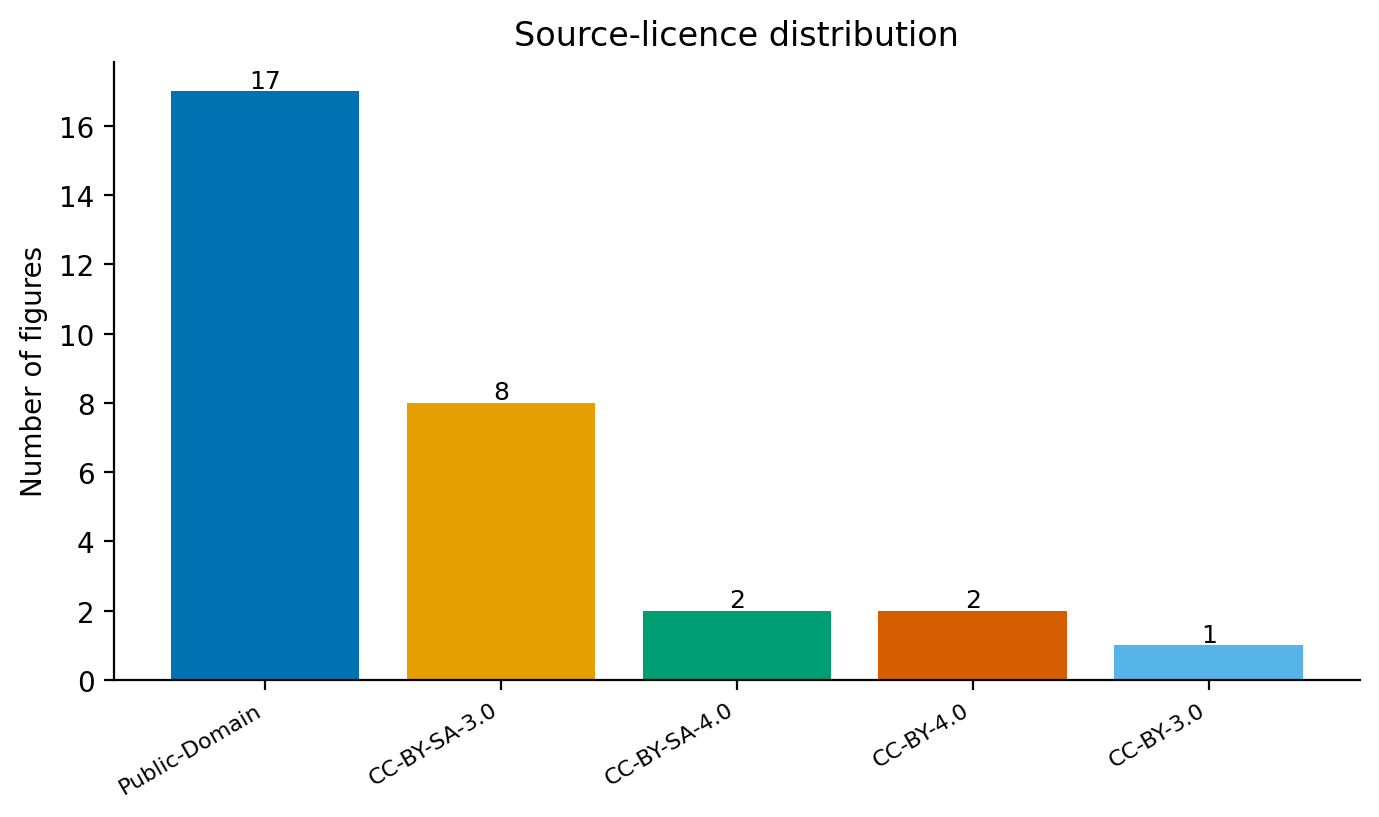
\includegraphics[width=0.86\textwidth]{fig3_licences.png}
\caption{Source-licence distribution across the 30 held-out figures. Bar chart: public domain 17, CC-BY-SA-3.0 8, CC-BY-SA-4.0 2, CC-BY-4.0 2, CC-BY-3.0 1. All figures are openly licensed, and the two CC-BY-4.0 figures are rendered locally and released by the author.}\label{fig:licences}
\end{figure}

\begin{figure}[!htb]
\centering
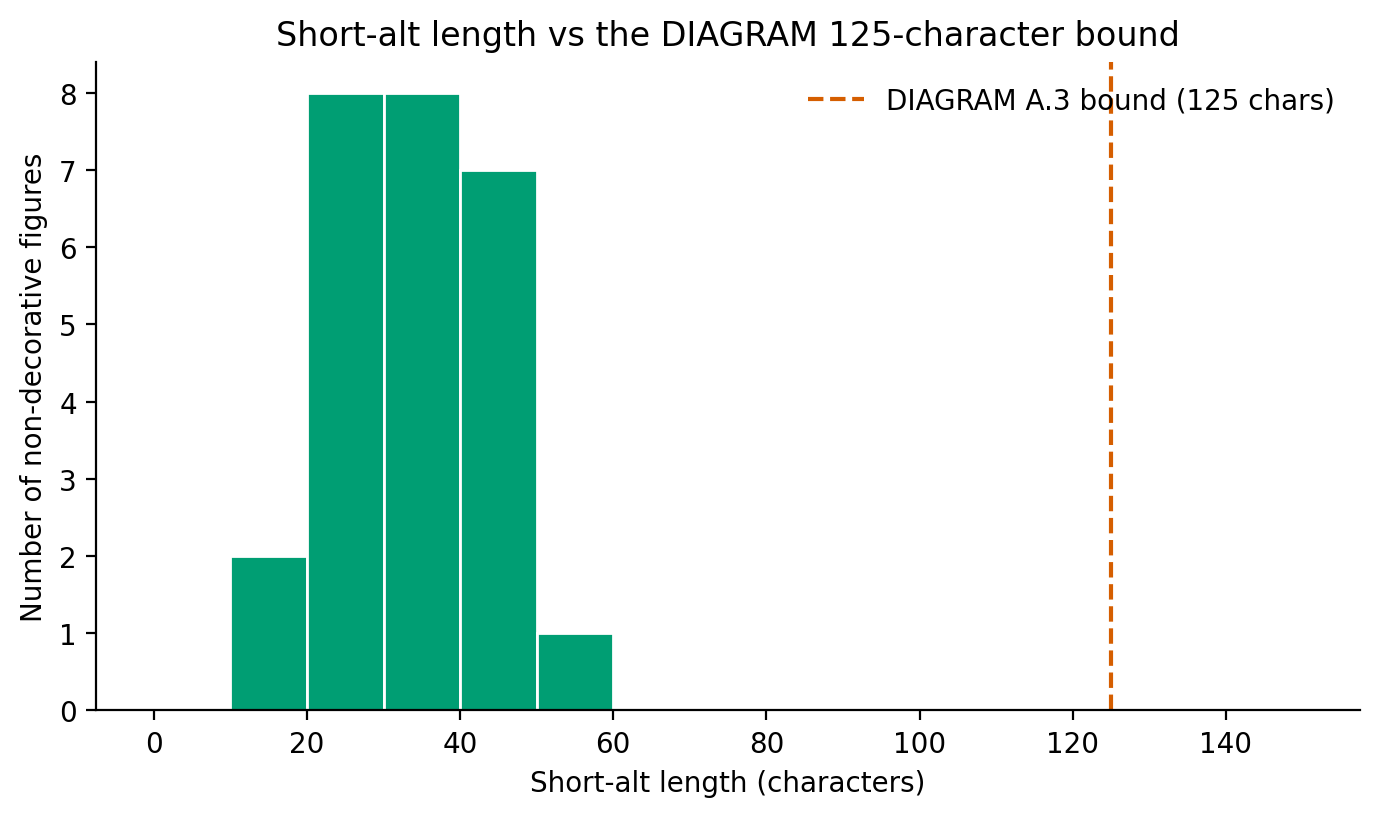
\includegraphics[width=0.86\textwidth]{fig4_short_alt_length.png}
\caption{Histogram of short-alt length for the 26 non-decorative figures, against the DIAGRAM \S A.3 125-character bound (dashed line). All short alts range from 17 to 53 characters (median 31.5) and sit well below the bound. The four decorative figures are excluded because their alt is empty by design, the correct WCAG handling of decorative images.}\label{fig:shortalt}
\end{figure}

%%%%%%%%%%%%%%%%%%%%%%%%%%%%%%%%%%%%%%%%%%%%%%%%%%%%%%%%%%%%%%%%%%%%%%
\section{Implementation, architecture, and reproducibility}\label{app:impl}
\setcounter{figure}{0}\setcounter{table}{0}

\subsection{Six-stage pipeline}\label{app:pipeline}

The reference implementation is a Python package (\texttt{stem\_alt}) and a six-stage Hydra pipeline. The stages run in order and share a single per-figure loop trace as the source of truth (Table~\ref{tab:pipeline}).

\begin{table}[!htb]
\caption{The six pipeline stages, with the artefact each reads and writes.}\label{tab:pipeline}
\centering
\footnotesize
\setlength{\tabcolsep}{4.5pt}
\begin{tabular}{clll}
\toprule
Stage & Script & Reads & Writes \\
\midrule
1 & \texttt{01\_build\_corpus.py} & \texttt{manifest.csv} & \texttt{splits.json} \\
2 & \texttt{02\_run\_loop.py} & calibration split & \texttt{loop\_traces/<id>.json} \\
3 & \texttt{03\_collect\_human\_ratings.py} & loop traces & \texttt{ratings\_*.jsonl} \\
4 & \texttt{04\_train\_dpo.py} & traces + ratings & \texttt{dpo/round\_NN/}, critic cfg \\
5 & \texttt{05\_evaluate.py} & held-out split + ratings & \texttt{held\_out\_report.json} \\
6 & \texttt{06\_release\_artefacts.py} & all of the above & born-accessible bundle \\
\bottomrule
\end{tabular}
\end{table}

\subsection{Factory/Registry pattern}\label{app:factory}

Each submodule under \texttt{src/stem\_alt/} (corpus, generator, critic, loop, training, evaluation, compliance, human) exposes a \texttt{<Type>Factory} lookup and a \texttt{register\_<type>(name)} decorator. A module-walk at import time fires the decorators without an explicit registration list. Adding a generator, critic, trainer, or compliance rule is then a one-file change with no edit to the factory wiring. Generators, critics, and trainers take a single \texttt{cfg} argument, and Hydra composes the config groups under \texttt{conf/<group>/<name>.yaml} at startup. Generator choice, LoRA rank, and DPO hyperparameters then sweep without code edits.

\subsection{Loop trace}\label{app:trace}

\texttt{LoopOrchestrator.run\_for\_figure} produces one \texttt{LoopRecord} per figure. The record holds the figure id, the list of rounds, a convergence flag, and the human score attached at stage 3. Each round carries its round index, the generation result with provenance, and the critic's five-dimension score. The trace is the single source of truth across stages 2 through 6, so re-running a stage reuses the snapshot rather than re-calling a model.

\subsection{Reproducibility contract}\label{app:repro}

STEM-Alt targets bit-exact reproducibility on the open-weights critic and full provenance on the closed-API generators. \texttt{utils.set\_seed} runs at the entry of every stage. It fixes \texttt{random}, \texttt{PYTHONHASHSEED}, NumPy, and Torch seeds, sets \texttt{cudnn.deterministic} true, and sets \texttt{cudnn.benchmark} false. The DPO trainer adds the round index so each fine-tuning round has a distinct seed. Hydra writes the resolved config tree to \texttt{outputs/<run>/.hydra/config.yaml}, the canonical record of the hyperparameters behind a checkpoint. Each stage also records the Python version, a frozen dependency list, the GPU model and driver, and the git commit and dirty-tree status. The corpus manifest is hashed with SHA-256 at stage 1, and the hash is written into the \texttt{splits.json} provenance block. Any change to a figure file or to the manifest then forces the splits to re-emit and the downstream stages to re-run. Two sources do not reproduce bit-exactly. Closed-API generation drifts across API versions; we mitigate this by logging the version string and snapshotting the output into the trace. Some non-deterministic CUDA kernels cause sub-1-ULP drift, mitigated by the deterministic-cuDNN setting and disclosed in \S\ref{sec:limitations}.

%%%%%%%%%%%%%%%%%%%%%%%%%%%%%%%%%%%%%%%%%%%%%%%%%%%%%%%%%%%%%%%%%%%%%%
\section{Compliance enforcement and born-accessible builds}\label{app:compliance}
\setcounter{figure}{0}\setcounter{table}{0}

Compliance is a gate, not an aspiration (\S\ref{sec:compliance}). The automated DIAGRAM linter rejects any gold-standard description that fails the rules at corpus-build time, and any loop output that fails them at rating time. The WCAG validator rejects any release HTML that fails Success Criterion 1.1.1 at release-bundle time. Table~\ref{tab:diagram-checklist} lists the seven DIAGRAM general rules and the check that enforces each.

\begin{table}[!htb]
\caption{DIAGRAM general-rule checklist and the corresponding linter check.}\label{tab:diagram-checklist}
\centering
\small
\begin{tabular}{p{0.30\textwidth}p{0.60\textwidth}}
\toprule
Rule & Linter check \\
\midrule
Context is key & The manifest must carry a non-empty context paragraph. \\
Audience-aware & Audience fixed at ``blind or low-vision STEM reader''; jargon density is checked against the figure's DIAGRAM type. \\
Be concise & Short alt $\leq 125$ characters where the image type permits. \\
Be objective & Pedagogical phrasing (``this teaches'', ``the goal of this figure'') is flagged. \\
General to specific & Every long description must open with a one-sentence summary, whose length is checked. \\
Tone & Passive constructions in long descriptions are flagged. \\
Inset handling & Graph insets are required to render as row-and-column tables in the long description (manually reviewed). \\
\bottomrule
\end{tabular}
\end{table}

At release time, \texttt{pipeline/06\_release\_artefacts.py} parses every \texttt{<img>} in the release HTML, builds a figure record, and runs the WCAG validator. Decorative images must declare \texttt{alt=""}, informative images must carry a non-empty \texttt{alt}, and complex images must reference a long description via \texttt{aria-describedby}. Any violation aborts the release. The tagged PDF is the primary born-accessible artefact. It is built by \texttt{pdflatex} and the SN template, and verified against PDF/UA with the PAC checker. Semantic HTML (audited with \texttt{axe-core} against WCAG 2.2 AA) and an EPUB3 build (audited with Ace by DAISY against EPUB Accessibility 1.1) are optional renderings produced from the same sources. The release pipeline refuses to ship a bundle in which any requested check failed.

%%%%%%%%%%%%%%%%%%%%%%%%%%%%%%%%%%%%%%%%%%%%%%%%%%%%%%%%%%%%%%%%%%%%%%
\section{Human-rating protocol}\label{app:human}
\setcounter{figure}{0}\setcounter{table}{0}

Two raters score each calibration figure. The first is a domain expert with research-level fluency in the figure's STEM area, recruited through ETH and MIT contacts and verified by institutional email or ORCID. The second is a screen-reader user, recruited first through Stiftung Zugang f\"ur alle, with a remote WAI-community rater as backup and a sighted rater with documented screen-reader experience as the disclosed fallback. Every record stores the rater's role, and fallback ratings are reported separately and excluded from the headline $\alpha$.

In a session, the rater receives the figure, its context paragraph, the DIAGRAM figure type, and the candidate alt-text, without the critic's scores, the generator identity, or the round index. Screen-reader-user raters listen to the alt-text rendered with NVDA at standard rate, live or from a pre-rendered WAV file. The rater scores each dimension 1 to 5 and writes a one-paragraph critique. Any score below 3 requires at least one supporting sentence. The session records the timestamp, an opaque rater id, the rater role, and an NVDA-rendering flag.

The five-dimension rubric is piloted on 20 figures and adjudicated pairwise. Differences of two or more points on any dimension are flagged, and the flagged pair adjudicates with the project lead present. The rubric definition is sharpened only when a disagreement reveals an ambiguity in the rubric rather than in the figure. The rubric is then frozen and committed. Any later edit is recorded as a protocol deviation in \S\ref{sec:limitations}. Headline statistics report two agreement numbers against their pre-registered thresholds. The $H_1$--$H_2$ inter-rater $\alpha$ is checked against the rating-quality floor of $0.6$ on the primary outcome. The $C$--$H$ $\alpha$ is checked against the convergence threshold of $0.7$ sustained across two consecutive DPO rounds. The gap between them bounds how far additional DPO data can push the critic without a richer rubric. A figure below the floor is adjudicated. If adjudication does not recover it, the figure leaves the calibration set and the exclusion is reported. The minimum-human-budget claim is the smallest count of fully two-rater-covered calibration figures at which the held-out threshold is reached. Human ratings carry no personally identifying information beyond the opaque rater id, and recruitment runs through institutional channels.

%%%%%%%%%%%%%%%%%%%%%%%%%%%%%%%%%%%%%%%%%%%%%%%%%%%%%%%%%%%%%%%%%%%%%%
\section{Evaluation harness and synthetic pipeline preview}\label{app:harness}
\setcounter{figure}{0}\setcounter{table}{0}

The evaluation harness (\texttt{analysis/generate\_eval\_figures.py}, covered by \texttt{tests/test\_eval\_figures.py}) renders four figures from the held-out report that \texttt{pipeline/05\_evaluate.py} writes: the convergence curve, the critic--human scatter, the per-dimension agreement bar chart, and the residual-disagreement heatmap defined in \S\ref{sec:eval}.

\begin{quote}
\textbf{The figures in this appendix are a synthetic pipeline preview, not a measured result.} No human rated these figures, no critic was trained, and no Krippendorff $\alpha$ was computed from real data. The values are generated by \texttt{code/scripts/generate\_synthetic\_ratings.py} (seed 20260604), the report carries a \texttt{\_SYNTHETIC} banner, and every rating line is tagged \texttt{"synthetic": true}. The preview exists only to exercise the report schema and the figure renderer end to end before the human study runs. The numbers must not be cited as findings, and \S\ref{sec:eval} reports the convergence $\alpha$ as a result only after the real study replaces this preview.
\end{quote}

The convergence curve and the critic--human scatter appear in the main text (\S\ref{sec:eval}, Figs~\ref{fig:demo-conv} and~\ref{fig:demo-scatter}). The two remaining shapes, the per-dimension agreement bar chart and the residual-disagreement heatmap, are shown here on the same synthetic report (Figs~\ref{fig:demo-perdim} and~\ref{fig:demo-resid}), so a reader can see the format the real study will fill.

\begin{figure}[!htb]
\centering
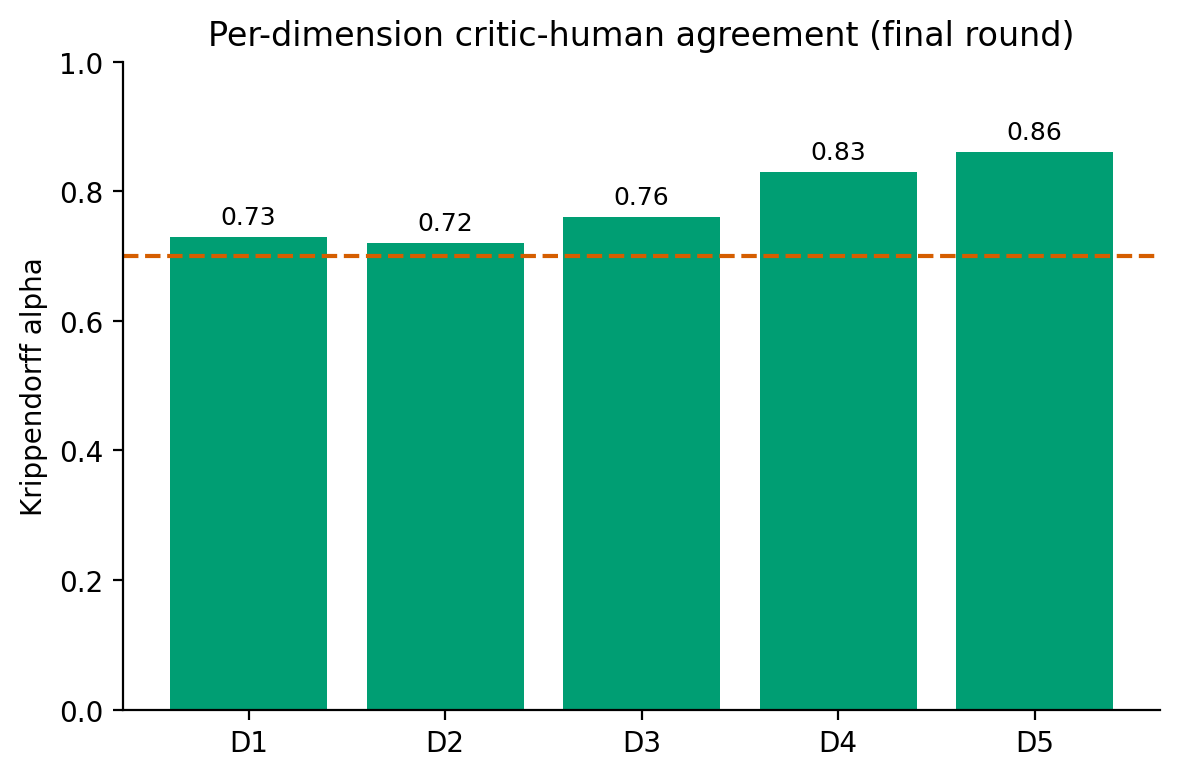
\includegraphics[width=0.78\textwidth]{fig_per_dimension.png}
\caption{Synthetic pipeline preview, not a measured result. Per-dimension agreement layout: the critic--human Krippendorff $\alpha$ for each rubric dimension ($D_1$--$D_5$) at the final round, against the $0.7$ reference line. Shape only; the values are simulated placeholders.}\label{fig:demo-perdim}
\end{figure}

\begin{figure}[!htb]
\centering
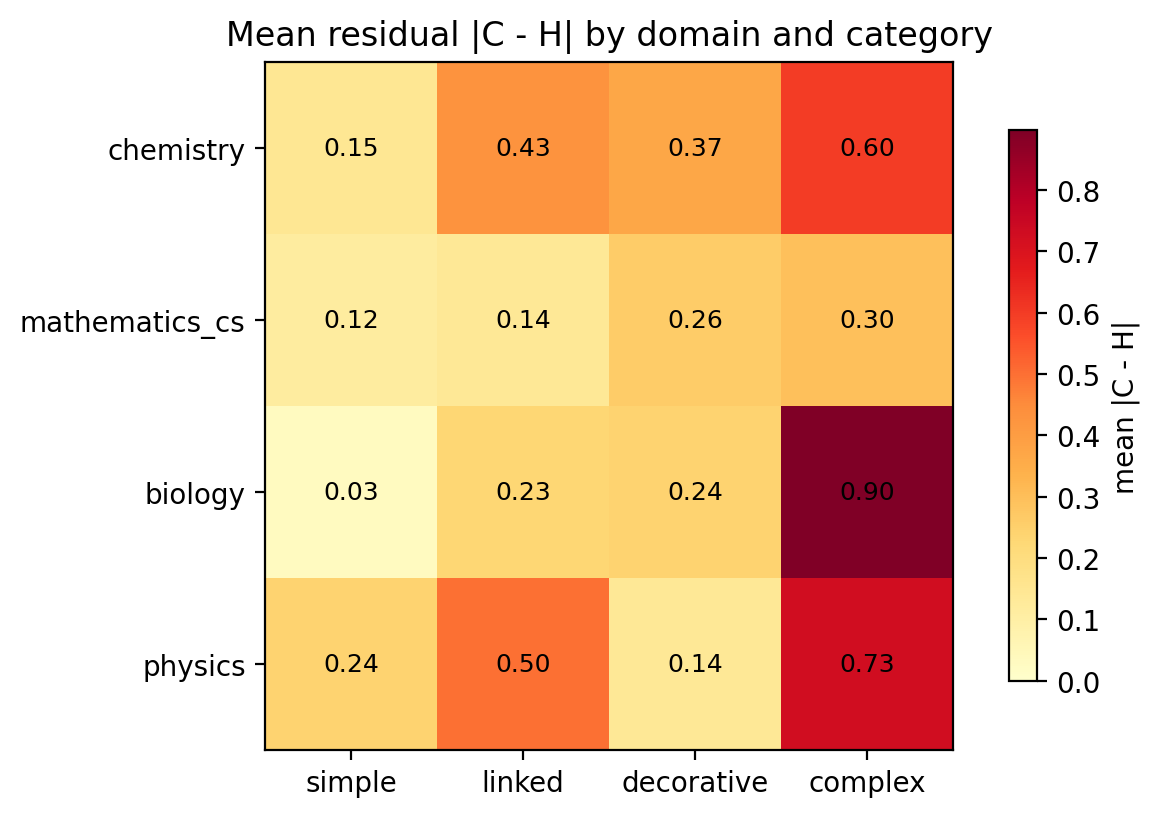
\includegraphics[width=0.78\textwidth]{fig_residual_heatmap.png}
\caption{Synthetic pipeline preview, not a measured result. Residual-disagreement heatmap layout: the mean absolute critic--human difference by STEM domain (rows) and ETH category (columns), with darker cells indicating larger disagreement. Shape only; the values are simulated placeholders.}\label{fig:demo-resid}
\end{figure}

\end{appendices}

\bibliography{references}

\end{document}
